\documentclass[11pt,a4paper]{report}

\usepackage[utf8]{inputenc}
\usepackage[T1]{fontenc}
\usepackage[french]{babel}
\usepackage{graphicx}
\usepackage{geometry}
\usepackage[table]{xcolor}
\usepackage{fancyhdr}
\usepackage{titlesec}
\usepackage{tocloft}
\usepackage{lastpage}
\usepackage[hidelinks]{hyperref}
\usepackage{longtable}
\usepackage{booktabs}
\usepackage{array}
\usepackage{enumitem}
\usepackage{placeins}

\geometry{margin=2.5cm}
\definecolor{orangeil}{RGB}{230,120,20}
\definecolor{tablehead}{RGB}{245, 226, 204}
\definecolor{tablerow}{RGB}{252, 246, 239}

\newcolumntype{L}[1]{>{\raggedright\arraybackslash}p{#1}}
\newcolumntype{C}[1]{>{\centering\arraybackslash}p{#1}}
\renewcommand{\arraystretch}{1.2}

\newcommand{\capture}[2]{
\begin{figure}[h]
\centering
\IfFileExists{#1}{
\includegraphics[width=\textwidth]{#1}
}{
\fbox{\parbox{0.92\textwidth}{\centering Capture manquante: #1}}
}
\caption{#2}
\end{figure}
}

% Header / Footer
\pagestyle{fancy}
\fancyhf{}
\fancyhead[C]{\textcolor{orangeil}{Rapport Projet IL S6}}
\fancyfoot[C]{\thepage\ /\ \pageref{LastPage}}
\renewcommand{\headrulewidth}{0.4pt}
\renewcommand{\footrulewidth}{0.4pt}
\fancypagestyle{plain}{
  \fancyhf{}
  \fancyhead[C]{\textcolor{orangeil}{Rapport Projet IL S6}}
  \fancyfoot[C]{\thepage\ /\ \pageref{LastPage}}
  \renewcommand{\headrulewidth}{0.4pt}
  \renewcommand{\footrulewidth}{0.4pt}
}
\setlength{\headheight}{15pt}

% Titres
\titleformat{\chapter}[block]{\Huge\bfseries\color{orangeil}}{\thechapter.}{10pt}{}
\titleformat{\section}{\Large\bfseries\color{orangeil}}{\thesection}{8pt}{}
\titleformat{\subsection}{\large\bfseries\color{orangeil}}{\thesubsection}{6pt}{}
\titlespacing*{\chapter}{0pt}{0pt}{18pt}
\titlespacing*{\section}{0pt}{10pt}{8pt}
\titlespacing*{\subsection}{0pt}{8pt}{6pt}

% Sommaire
\renewcommand{\contentsname}{\textcolor{orangeil}{Sommaire}}
\renewcommand{\cftchapfont}{\color{orangeil}\bfseries}
\renewcommand{\cftchappagefont}{\color{orangeil}\bfseries}
\renewcommand{\cftchapleader}{\cftdotfill{\cftdotsep}}
\renewcommand{\cftsecfont}{\color{orangeil}}
\renewcommand{\cftsecpagefont}{\color{orangeil}}
\renewcommand{\cftsecleader}{\cftdotfill{\cftdotsep}}
\setlength{\cftbeforechapskip}{8pt}
\setlength{\cftbeforesecskip}{4pt}

\begin{document}

% Page de garde
\begin{titlepage}
\begin{center}
\vspace*{1cm}

\includegraphics[width=5cm]{logo-avignon.jpg}

\vspace{1.5cm}

{\Huge \bfseries Rapport Final \par}
\vspace{0.3cm}
{\Large Projet IL 2025--2026 \par}
\vspace{0.8cm}

{\LARGE \textbf{Plateforme collaborative de visionnage vidéo} \par}
\vspace{0.3cm}
{\LARGE \textbf{WithYou - Régie Vidéo (Cycle 3)} \par}

\vspace{1.5cm}

{\large Université d'Avignon \par}
{\large \today \par}

\vspace{2cm}

\begin{tabular}{p{6cm} p{6cm}}
\textbf{Prestataires :} & \textbf{Clients :} \\
Takdjerad Meriem & KESSLER Rémy \\
Ghabi Malek & BONNEFOY Ludovic \\
Taleb Wissame & \\
Taleb Lamia & \\
Laftimi Yanis & \\
\end{tabular}

\vfill
{\small UFR Sciences, Technologies, Santé --- CERI}
\end{center}
\end{titlepage}

\setcounter{page}{1}
\addcontentsline{toc}{chapter}{Page de garde}
\tableofcontents
\newpage

\chapter{Introduction}
\section{Contexte}
Le projet \textit{WithYou} est initialement issu d'un MVP centré sur le visionnage vidéo collaboratif. Ce socle fonctionnel, validé lors des premières phases du projet, permettait déjà la diffusion synchronisée et l'interaction de base entre participants.

Dans le cadre du présent semestre, le produit a été réorienté vers un usage plus exigeant, où la notion de \textit{régie} devient centrale. L'objectif n'est plus uniquement de regarder une vidéo à plusieurs, mais de piloter une séance complète : organiser les transitions, encadrer les interventions, superviser l'engagement des participants et conserver une traçabilité des actions réalisées.

Cette évolution concerne en particulier des contextes pédagogiques, d'animation de communauté et de diffusion encadrée, dans lesquels la qualité de coordination en temps réel est déterminante. Le défi principal du semestre a donc consisté à faire évoluer l'architecture existante vers une version plus robuste et plus outillée, sans dégrader la stabilité globale de l'application.

\section{Objectif du rapport}
Ce rapport final a pour objectif de présenter, de manière structurée et argumentée, le cheminement complet suivi entre le cycle 1 et le cycle 3. Il met en évidence la continuité des décisions prises, les arbitrages réalisés en cours de développement et la manière dont les risques identifiés ont été traités.

Le document est organisé autour de trois axes complémentaires :
\begin{itemize}
    \item une synthèse de la logique de progression entre les cycles (exploration, prototypage, finalisation) ;
    \item une analyse détaillée des contributions par membre, avec pour chaque fonctionnalité les risques rencontrés, les choix techniques, les difficultés et les solutions apportées ;
    \item une validation globale de la version finale, appuyée par des scénarios de test, une matrice de traçabilité et des éléments de preuve technique.
\end{itemize}

\section{Méthode en spirale}
La conduite du projet s'appuie sur la méthode en spirale, adaptée au cadre pédagogique du module. Cette approche repose sur une progression itérative dans laquelle chaque cycle est guidé en priorité par la réduction des risques, et non par l'accumulation rapide de fonctionnalités.

Chaque cycle suit un enchaînement clair :
\begin{enumerate}
    \item définition des objectifs du cycle et du périmètre de travail ;
    \item identification et priorisation des risques (techniques, fonctionnels, UX, organisationnels) ;
    \item expérimentation et implémentation ciblées pour lever les risques majeurs ;
    \item analyse des résultats et décision pour la suite (valider, ajuster, reporter).
\end{enumerate}

Cette logique a permis de sécuriser progressivement l'évolution de \textit{WithYou} : d'abord en validant l'orientation produit, ensuite en éprouvant les briques critiques du temps réel, puis en consolidant une version finale stable et exploitable. La méthode en spirale a ainsi servi de cadre de décision tout au long du projet, en maintenant un lien constant entre risques identifiés, implémentations réalisées et niveau de maturité obtenu.

\chapter[Synthèse cycles précédents]{Synthèse des cycles précédents}
\section[Cycle 1 : choix de la piste]{Cycle 1 : choix de la piste et risques stratégiques}
Le cycle 1 avait une vocation principalement exploratoire : comparer les pistes d'évolution possibles du MVP et identifier, pour chacune, les risques majeurs avant tout investissement technique lourd. Trois orientations ont été étudiées de manière structurée :
\begin{itemize}
    \item \textbf{Piste 1 -- Mode Cours interactif}, à forte valeur pédagogique mais exigeante en termes de complexité fonctionnelle ;
    \item \textbf{Piste 2 -- Régie Vidéo avancée}, centrée sur le pilotage de séance en temps réel ;
    \item \textbf{Piste 3 -- Plateforme de formation sécurisée}, orientée gestion d'accès et cadrage académique.
\end{itemize}

La comparaison a porté sur les risques stratégiques, techniques et fonctionnels de chaque piste. Le risque principal du cycle 1 était un \textbf{risque d'orientation} : sélectionner une direction inadaptée au public cible ou au niveau de maturité de la plateforme.

À l'issue de cette analyse, la piste \textbf{Régie Vidéo} a été retenue comme axe principal, car elle apportait la meilleure cohérence entre valeur d'usage, faisabilité progressive et potentiel d'enrichissement collaboratif. La dimension « plateforme sécurisée » a été conservée comme axe complémentaire, à intégrer de façon progressive.

\section[Cycle 2 : prototype validé]{Cycle 2 : prototype et risques techniques levés}
Le cycle 2 avait pour objectif de valider techniquement les choix du cycle 1 à travers un prototype fonctionnel. L'effort s'est concentré sur les briques critiques :
\begin{itemize}
    \item régie vidéo (lecture, pause, navigation temporelle, changement de vidéo, playlist) ;
    \item synchronisation multi-clients via diffusion d'événements temps réel ;
    \item gestion des rôles et permissions (professeur, régie, étudiant) ;
    \item authentification et premières contraintes de sécurisation des accès.
\end{itemize}

Le \textbf{risque majeur} du cycle 2 concernait la fiabilité de la synchronisation vidéo en conditions réelles (latence, propagation des événements, cohérence d'état entre clients). Les expérimentations ont montré une faisabilité globale satisfaisante : les actions de régie et les mécanismes de diffusion synchronisée sont devenus opérationnels, avec quelques décalages résiduels identifiés.

Sur le plan organisationnel, le cycle 2 a également permis de structurer les permissions en temps réel et de poser une base d'authentification exploitable pour la suite. Ces résultats ont validé l'orientation retenue au cycle 1 et ont fourni une base solide pour la finalisation.

\section{Transition vers le cycle 3}
À la fin du cycle 2, les choix technico-fonctionnels étaient validés, mais plusieurs points critiques restaient à traiter avant une version finale :
\begin{itemize}
    \item stabilisation des flux realtime et réduction des écarts de synchronisation ;
    \item enrichissement des outils de régie (pilotage avancé, supervision, interaction) ;
    \item amélioration de la robustesse réseau (reconnexion, reprise d'état, gestion d'erreurs) ;
    \item consolidation de la cohérence d'expérience entre les différents rôles utilisateurs.
\end{itemize}

Le cycle 3 a donc été planifié comme un cycle de \textbf{finalisation et de stabilisation} : transformer le prototype validé en une version exploitable, mieux documentée, testée et soutenable en démonstration complète.

\chapter{Cycle 3 : objectifs et périmètre final}
\section{Objectifs du cycle 3}
Le cycle 3 correspond à la phase de finalisation : transformer le prototype du cycle 2 en une version stable, cohérente et démontrable.

Les objectifs principaux sont :
\begin{itemize}
    \item finaliser les fonctionnalités avancées de régie ;
    \item stabiliser l'application (realtime, erreurs réseau, reconnexion, cohérence d'état) ;
    \item livrer une version exploitable en séance complète.
\end{itemize}

\section{Fonctionnalités visées en version finale}
Le périmètre fonctionnel du cycle 3 a été défini à partir des risques résiduels identifiés en sortie du cycle 2 et des besoins prioritaires de la piste Régie Vidéo. L'objectif a été de couvrir l'ensemble des mécanismes nécessaires à une séance pilotée en temps réel, sans rupture de synchronisation et avec un niveau de contrôle suffisant pour la régie.

Le périmètre final inclut notamment :
\begin{itemize}
    \item la \textbf{gestion dynamique de diffusion} (vote vidéo en temps réel, transitions entre contenus, changement de scène) ;
    \item les \textbf{outils de pilotage régie} (annonces, supervision des participants, verrouillage de session, historique des actions) ;
    \item les \textbf{mécanismes de modération et d'interaction} (permissions individuelles, demandes de parole, questions post-vidéo, sondages) ;
    \item les \textbf{composants de synchronisation avancée} (reprise automatique, recalage des clients, cohérence des états lecture/pause/temps) ;
    \item les \textbf{extensions d'assistance IA} (génération de contenu, appui à l'animation de discussion, enrichissement contextuel).
\end{itemize}

Ce périmètre a été construit avec une logique de cohérence produit : chaque fonctionnalité devait s'intégrer dans la chaîne complète de pilotage de séance et non exister de manière isolée.

\section{Critères de réussite}
Les critères de validation retenus pour le cycle 3 sont les suivants :
\begin{itemize}
    \item \textbf{stabilité multi-utilisateurs} : fonctionnement correct avec plusieurs participants connectés ;
    \item \textbf{cohérence régie/spectateurs} : états lecture/pause/temps/transitions alignés ;
    \item \textbf{fonctionnalités critiques finalisées} : modules essentiels implémentés et testés ;
    \item \textbf{documentation claire} : limites restantes et actions en cours explicitement indiquées.
\end{itemize}

\chapter{Démarche et répartition des tâches}
\section{Méthodologie appliquée}
Le pilotage S6 a suivi la logique de la méthode en spirale en trois cycles :
\begin{itemize}
    \item \textbf{Cycle 1} : cadrage, comparaison des pistes et choix argumenté.
    \item \textbf{Cycle 2} : prototypage des mécanismes critiques (régie, realtime, permissions).
    \item \textbf{Cycle 3} : finalisation, stabilisation, tests d'intégration et préparation du rendu.
\end{itemize}

\section{Répartition des rôles}
\begin{itemize}
    \item \textbf{Régie / Frontend interactif} : Malek, Meriem, Lamia.
    \item \textbf{Fonctions de modération et pilotage de séance} : Wissame.
    \item \textbf{Supervision d'activité et export de séance} : Yanis.
    \item \textbf{Tests d'intégration, validation et documentation} : équipe complète.
\end{itemize}

\section{Répartition détaillée des tâches par cycle}
Les tableaux ci-dessous présentent une \textbf{vue générale} de la répartition par cycle.  
Le \textbf{suivi détaillé des tâches} (granularité fine, dates et enchaînements complets) est fourni en annexe dans la section dédiée au suivi.

\subsection{Cycle 1 --- Exploration et choix de piste}
\rowcolors{2}{tablerow}{white}
\begin{longtable}{L{0.28\textwidth} L{0.60\textwidth}}
\toprule
\rowcolor{tablehead}
\textbf{Phase} & \textbf{Tâche} \\
\midrule
Pilotage équipe & Lancement S6, répartition en sous-groupes, plan de travail \\
Analyse MVP & Audit front/back/realtime et contraintes techniques/UX \\
Étude pistes & Étude des 3 pistes + matrice de risques par piste \\
Arbitrage & Comparaison globale et décision : piste Régie principale \\
Documentation & Rédaction, relecture et dépôt du rapport cycle 1 \\
\bottomrule
\end{longtable}

\subsection{Cycle 2 --- Prototype}
\rowcolors{2}{tablerow}{white}
\begin{longtable}{L{0.28\textwidth} L{0.60\textwidth}}
\toprule
\rowcolor{tablehead}
\textbf{Phase} & \textbf{Tâche} \\
\midrule
Architecture & Définition architecture du prototype cycle 2 \\
Régie v1 & Contrôles play/pause/seek + changement vidéo \\
Realtime & Broadcast état vidéo + recalage spectateurs \\
Playlist & CRUD playlist et gestion vidéo courante \\
Auth/Rôles & Auth Supabase + rôles initiaux + permissions de base \\
UI/UX & Refonte partielle de l'interface régie \\
QA + correctifs & Tests techniques du prototype + corrections critiques \\
Documentation & Rédaction et dépôt du rapport cycle 2 \\
\bottomrule
\end{longtable}

\subsection{Cycle 3 --- Version finale}
\rowcolors{2}{tablerow}{white}
\begin{longtable}{L{0.28\textwidth} L{0.60\textwidth}}
\toprule
\rowcolor{tablehead}
\textbf{Bloc} & \textbf{Tâches principales} \\
\midrule
Régie avancée & Vote 5 min, sélection auto gagnant, transitions, countdown, annonces, historique, preview privée, bookmarks, \texttt{-10s/+10s} \\
Audio live & Voix live régie WebRTC + stabilisation SDP/ICE \\
Interaction avancée & Mode Director, zoom partagé, question post-vidéo, demandes de parole \\
IA de contenu & Aperçu IA vidéo, questions IA, contenu du salon, transcription/captions \\
Permissions v2 & Permissions granulaires finales + propagation realtime \\
Fiabilité & Gestion erreurs réseau, erreurs 400 et fallback \\
Intégration Git & Résolution conflits et réintégration features \\
QA final & Tests E2E + corrections non-régression \\
Documentation / rendu & Mise à jour docs + préparation soutenance + rendu final \\
\bottomrule
\end{longtable}

\subsection{Travail collectif}
\rowcolors{2}{tablerow}{white}
\begin{longtable}{L{0.30\textwidth} C{0.18\textwidth} L{0.42\textwidth}}
\toprule
\rowcolor{tablehead}
\textbf{Action collective} & \textbf{Fréquence} & \textbf{Résultat} \\
\midrule
Réunions de pilotage & Hebdomadaire & Arbitrages fonctionnels validés \\
Tests croisés inter-membres & Continue & Réduction des régressions d'intégration \\
Revue des risques & Fin de cycle & Priorisation cohérente des correctifs \\
Documentation commune & Continue & Alignement rapport, README et preuves techniques \\
\bottomrule
\end{longtable}

\chapter{Contributions individuelles détaillées}

\section{Membre 1 -- Taleb Lamia}
\subsection{Risques rencontrés}
\begin{itemize}
    \item \textbf{Risque pédagogique :} absence de transition structurée entre le visionnage et l'échange collectif.
    \item \textbf{Risque organisationnel :} interventions simultanées sans mécanisme de demande de parole.
    \item \textbf{Risque fonctionnel :} forte dépendance aux actions manuelles de la régie sans orchestration de séance.
\end{itemize}
\subsection{Implémentation détaillée}
\paragraph{1. Question après vidéo (\textit{Fait})}
Taleb Lamia a ajouté un mécanisme permettant à la régie de préparer une question liée à la vidéo en cours, puis de l'afficher automatiquement à la fin de la lecture. Cette fonctionnalité crée une transition immédiate vers la discussion et améliore l'usage pédagogique de la plateforme en proposant un point de réflexion au bon moment.

\paragraph{2. Lever la main / demandes de parole (\textit{Partiel})}
Une fonctionnalité de demande de parole a été intégrée : les participants peuvent signaler qu'ils souhaitent intervenir, et la régie visualise les demandes en attente pour organiser l'ordre de prise de parole. La contribution précise explicitement la limite actuelle : la signalisation est opérationnelle, mais l'activation d'une vraie prise de parole audio automatisée n'est pas finalisée.

\paragraph{3. Programme régie (\textit{En cours})}
Taleb Lamia a commencé un module de programme régie visant à préparer un enchaînement automatique d'étapes de séance (exemple : annonce, compte à rebours, lancement vidéo). L'objectif est de réduire les manipulations répétitives et de rapprocher l'application d'un fonctionnement de régie professionnelle.
\subsection{Difficultés / solutions}
La principale difficulté rencontrée concerne l'extension de la demande de parole vers un flux audio complet. En l'état, la logique de gestion de file est valide, mais l'intégration micro/voix participant reste un chantier de finalisation identifié pour la suite.
\subsection{Statut}
\begin{itemize}
    \item Question après vidéo : \textbf{Fait}
    \item Lever la main / demandes de parole : \textbf{Partiel}
    \item Programme régie : \textbf{En cours}
\end{itemize}
\subsection{Captures d'écran associées}
\capture{captures/lamia-question-apres-video.png}{Question après vidéo}
\capture{captures/lamia-demandes-parole.png}{Demandes de parole}
\capture{captures/lamia-programme-regie.png}{Programme régie}
\FloatBarrier

\section{Membre 2 -- Takdjerad Meriem}
\subsection{Risques rencontrés}
\begin{itemize}
    \item \textbf{Risque de pilotage temporel insuffisant :} sans contrôle fin, la régie ne peut pas adapter rapidement le rythme de diffusion à la séance.
    \item \textbf{Risque de guidage visuel limité :} absence d'annotation live pour attirer l'attention sur un détail précis.
    \item \textbf{Risque d'engagement faible :} interaction réduite sans mécanisme de sondage collectif en temps réel.
\end{itemize}
\subsection{Implémentation détaillée}
\paragraph{1. Contrôle de lecture avancé et navigation synchronisée (\textit{Fait})}
Meriem a implémenté un contrôle de lecture précis avec deux actions dédiées : retour arrière de dix secondes et avance rapide de dix secondes. Lorsqu'une action est déclenchée, le système calcule la nouvelle position cible puis applique un bornage pour empêcher toute valeur négative ou supérieure à la durée du média. La mise à jour est propagée à tous les participants via la synchronisation temps réel, ce qui conserve une lecture partagée cohérente.

\paragraph{2. Mode Director et annotations en temps réel (\textit{Fait})}
Le Mode Director repose sur un \textit{canvas} superposé au lecteur vidéo, sans altérer le player existant. La régie peut dessiner en direct et les tracés sont transmis instantanément à l'ensemble des participants. Un mécanisme de réinitialisation globale permet d'effacer toutes les annotations en une seule action.

\paragraph{3. Système de sondage interactif assisté par IA (\textit{Fait})}
Le module de sondage inclut deux modes :
\begin{itemize}
    \item un mode manuel (question, choix, durée),
    \item un mode assisté par IA (génération contextualisée à partir de la vidéo en cours).
\end{itemize}
Le sondage est diffusé simultanément à tous les participants, avec vote unique par utilisateur, agrégation des réponses en temps réel et possibilité d'arrêt anticipé par la régie.
\subsection{Difficultés / solutions}
Les principales difficultés ont concerné :
\begin{itemize}
    \item le bornage robuste des sauts temporels pour garantir des positions valides ;
    \item la synchronisation des annotations sans perturber le lecteur principal ;
    \item la cohérence du flux de sondage (unicité des votes et actualisation instantanée des résultats).
\end{itemize}
\subsection{Statut}
\begin{itemize}
    \item Contrôle avancé \texttt{-10s/+10s} : \textbf{Fait}
    \item Mode Director : \textbf{Fait}
    \item Sondage interactif assisté par IA : \textbf{Fait}
\end{itemize}
\subsection{Captures d'écran associées}
\capture{captures/meriem-jump-controls.png}{Contrôle avancé \texttt{-10s/+10s}}
\capture{captures/meriem-mode-director.png}{Mode Director}
\capture{captures/meriem-sondage-ia.png}{Sondage IA}
\FloatBarrier

\section{Membre 3 -- Taleb Wissame}
\subsection{Risques rencontrés}
\begin{itemize}
    \item \textbf{Risque de perte de repères vidéo :} difficulté à revenir rapidement sur un passage important sans navigation contextuelle.
    \item \textbf{Risque de dérive du cadre de séance :} manque d'outils de contrôle global pour organiser les phases d'écoute et d'échange.
    \item \textbf{Risque de manque de traçabilité :} impossibilité de relire clairement les actions de régie après une séance longue.
    \item \textbf{Risque de communication peu lisible :} messages importants noyés dans le chat conversationnel.
    \item \textbf{Risque de pilotage pédagogique faible :} absence de retour immédiat sur la compréhension des participants.
\end{itemize}
\subsection{Implémentation détaillée}
\paragraph{1. Marque-pages vidéo et navigation contextuelle (\textit{Fait})}
Un système de marque-pages a été mis en place pour associer à un instant précis de la vidéo un horodatage, un libellé et l'identité du créateur. Cette fonctionnalité permet de retrouver rapidement un passage clé, de structurer la relecture et de renforcer l'usage pédagogique (explication ciblée, retour sur extrait, support de question).

\paragraph{2. Verrouillage de session et maîtrise de l'environnement (\textit{Fait})}
Le module de verrouillage regroupe plusieurs leviers de régulation : verrouillage de salle, désactivation temporaire du chat et mode focus. L'objectif est de mieux contrôler l'environnement de séance, de limiter les distractions et de conserver une dynamique de groupe lisible.

\paragraph{3. Baromètre de compréhension en temps réel (\textit{Fait})}
Le baromètre permet aux participants d'envoyer des signaux simples (\textit{compris}, \textit{ralentir}, \textit{perdu}). Les retours sont agrégés afin d'offrir à la régie une vue synthétique du ressenti du groupe et d'ajuster immédiatement le rythme de diffusion.

\paragraph{4. Historique des actions de régie (\textit{Fait})}
Un historique horodaté des actions régie a été intégré (annonces, marque-pages, changements d'état). Il améliore la traçabilité opérationnelle, facilite l'analyse a posteriori et participe à une logique d'audit léger des séances.

\paragraph{5. Système d'annonces et communication prioritaire (\textit{Fait})}
Un canal d'annonces a été conçu pour distinguer les messages organisationnels des échanges ordinaires du chat. La régie peut diffuser une information prioritaire, visible immédiatement par tout le groupe (consigne, reprise, changement de déroulement).
\subsection{Difficultés / solutions}
\begin{itemize}
    \item Arbitrer entre richesse fonctionnelle et simplicité visuelle de l'interface.
    \item Organiser la coexistence entre communication libre (chat) et communication de pilotage (annonces).
    \item Conserver une logique de régulation pédagogique sans alourdir l'expérience utilisateur.
\end{itemize}
\subsection{Statut}
\begin{itemize}
    \item Marque-pages vidéo : \textbf{Fait}
    \item Verrouillage de session : \textbf{Fait}
    \item Baromètre de compréhension : \textbf{Fait}
    \item Historique des actions de régie : \textbf{Fait}
    \item Système d'annonces régie : \textbf{Fait}
\end{itemize}
\subsection{Captures d'écran associées}
\capture{captures/wissame-bookmarks.png}{Marque-pages vidéo}
\capture{captures/wissame-session-lock.png}{Verrouillage de session}
\capture{captures/wissame-annonces-historique.png}{Annonces et historique régie}
\FloatBarrier

\section{Membre 4 -- Malek Ghabi}
\subsection{Risques rencontrés}
\begin{itemize}
    \item \textbf{Risque de désynchronisation multi-clients} lors des votes, des comptes à rebours et des changements d'état.
    \item \textbf{Risque de stabilité realtime} (erreurs 400, boucles de reconnexion, concurrence d'événements).
    \item \textbf{Risque d'expérience dégradée} sur les transitions vidéo, le son live et les aperçus dynamiques de playlist.
    \item \textbf{Risque de sécurité fonctionnelle} sur les permissions individuelles (contournement côté client).
    \item \textbf{Risque d'échec partiel IA} (latence, réponses incomplètes, JSON vide).
\end{itemize}
\subsection{Implémentation détaillée}
\paragraph{1. Vote vidéo en temps réel (\textit{Fait})}
Panneau de vote collaboratif diffusé en temps réel avec agrégation centralisée et sélection automatique de la vidéo gagnante en fin de minuterie.

\paragraph{2. Compte à rebours partagé (\textit{Fait})}
Décompte commun synchronisé (\texttt{3...2...1...GO}) basé sur un timestamp absolu pour garantir un démarrage homogène sur tous les clients.

\paragraph{3. Transitions entre vidéos (\textit{Fait})}
Intégration des transitions visuelles (\textit{Cut}, \textit{Fondu noir}, \textit{Glissement}, \textit{Flash blanc}) avec déclenchement coordonné au changement de média.

\paragraph{4. Voix live régie (\textit{En cours})}
Diffusion micro régie en temps réel via WebRTC. La fonctionnalité est opérationnelle et en cours de stabilisation sur les cas réseau dégradés.

\paragraph{5. Annonces vocales TTS (\textit{Fait})}
Diffusion d'annonces vocales synthétiques à l'ensemble du salon avec fallback texte côté interface.

\paragraph{6. Permissions individuelles en temps réel (\textit{Fait})}
Gestion granulaire des droits par participant avec propagation instantanée des changements et contrôle côté exécution.

\paragraph{7. Synchronisation et reprise automatique (\textit{Fait})}
Synchronisation maître-esclave avec recalage automatique à la reconnexion selon l'état courant de la régie.

\paragraph{8. Playlist enrichie au survol (\textit{En cours})}
Aperçu contextuel au survol (titre complet + preview courte) avec chargement dynamique pour limiter la consommation client.

\paragraph{9. Modes d'affichage de session (\textit{Fait})}
Pilotage centralisé des layouts (\textit{Cinema}, \textit{Split}, \textit{Party}, \textit{Interlude}) avec propagation immédiate au groupe.

\paragraph{10. Fonctions IA de contenu (\textit{Fait})}
Intégration de fonctions IA (preview, contenu de salon, questions, transcription/captions) avec gestion des états de chargement et fallback UI.
\subsection{Difficultés / solutions}
\begin{itemize}
    \item Gestion de la concurrence d'événements realtime et réduction du bruit réseau.
    \item Stabilisation progressive du canal audio live (WebRTC) en environnement multi-clients.
    \item Arbitrage entre fluidité UX et robustesse technique (transitions, overlays, synchronisation).
\end{itemize}
\subsection{Statut}
\begin{itemize}
    \item Finalisées : vote, countdown, transitions, TTS, permissions, synchronisation/reprise, modes d'affichage, IA.
    \item En cours : voix live régie, playlist enrichie au survol.
\end{itemize}
\subsection{Captures d'écran associées}
\capture{captures/malek-vote-realtime.png}{Vote vidéo en temps réel}
\capture{captures/malek-countdown-shared.png}{Compte à rebours partagé}
\capture{captures/malek-video-transitions.png}{Transitions entre vidéos}
\capture{captures/malek-live-voice-regie.png}{Voix live régie}
\capture{captures/malek-tts-annonce.png}{Annonces vocales TTS}
\capture{captures/malek-permissions-individuelles.png}{Permissions individuelles}
\capture{captures/malek-sync-reprise-auto.png}{Synchronisation et reprise}
\capture{captures/malek-playlist-hover-preview.png}{Playlist enrichie au survol}
\capture{captures/malek-scene-modes.png}{Modes d'affichage de la session}
\capture{captures/malek-ia-contenu-session.png}{Fonctions IA de contenu}
\FloatBarrier

\section{Membre 5 -- Laftimi Yanis}
\subsection{Risques rencontrés}
\begin{itemize}
    \item \textbf{Risque de perte de supervision régie :} absence d'indicateurs d'engagement en temps réel sur les participants.
    \item \textbf{Risque de faible traçabilité post-session :} manque d'outil de synthèse exportable pour conserver les événements d'une séance.
\end{itemize}
\subsection{Implémentation détaillée}
\paragraph{1. Détection d'inactivité et alertes régie en temps réel (\textit{Fait})}
Yanis a implémenté un système de suivi d'activité participant basé sur des pings d'interaction (souris, clavier, clic, scroll), avec \textit{debounce} de 30 secondes pour éviter la surcharge du canal realtime. Côté régie, chaque utilisateur est reclassifié périodiquement en \textit{actif} (\(<2\) min), \textit{inactif} (2--5 min) ou \textit{AFK} (\(>5\) min). L'état est rendu visuellement par un badge coloré et une notification toast est envoyée lors d'un basculement AFK. Un bouton « Notifier les AFK » permet d'envoyer un rappel ciblé.

\textbf{Bénéfice :} supervision immédiate de l'engagement et meilleure réactivité d'animation.

\paragraph{2. Export automatisé du rapport de session en PDF (\textit{Fait})}
Une fonction d'export PDF côté client a été ajoutée via \texttt{jsPDF} et \texttt{html2canvas}. Un composant React invisible (\texttt{SessionReportTemplate}) est rendu temporairement, puis capturé et paginé automatiquement en format A4. Les données incluent les informations de salon, participants, vidéos diffusées, actions régie et signets, avec récupération via Supabase et hook dédié.

\textbf{Bénéfice :} création d'un compte-rendu exploitable pour audit, pédagogie et suivi post-session.

\subsection{Difficultés / solutions}
\begin{itemize}
    \item Éviter le bruit réseau de supervision : résolution par \textit{debounce} des pings et reclassification par intervalle.
    \item Générer un PDF riche sans backend dédié : résolution via rendu React hors écran + capture haute résolution + pagination automatique.
\end{itemize}
\subsection{Statut}
\begin{itemize}
    \item Détection d'inactivité et alertes régie : \textbf{Fait}
    \item Export automatisé de rapport PDF : \textbf{Fait}
\end{itemize}
\subsection{Captures d'écran associées}
\capture{captures/yanis-inactivite-alertes.png}{Détection d'inactivité et alertes régie}
\capture{captures/yanis-export-session-pdf.png}{Export automatisé du rapport de session}
\FloatBarrier

\chapter{Tests et validation}

\section{Stratégie de test}
Les tests ont été réalisés en conditions proches du réel, avec plusieurs clients connectés (régie, membres, invités). L'objectif était de valider la stabilité, la synchronisation et les outils de régie.
\begin{itemize}
    \item \textbf{Tests fonctionnels} : vérification des fonctionnalités une par une.
    \item \textbf{Tests d'intégration} : vérification de la cohérence entre les modules.
    \item \textbf{Tests de résilience} : coupures réseau, reconnexions, erreurs realtime.
    \item \textbf{Tests UX} : lisibilité des retours visuels et facilité d'usage.
\end{itemize}

\section{Scénarios testés}
Les scénarios suivants ont été exécutés pour vérifier le fonctionnement global de la séance.

\begin{enumerate}
    \item \textbf{Concertation et choix de média (Vote vidéo en temps réel) :} L'ouverture d'un vote par l'administrateur, suivie de participations multiples, a abouti à une élection conforme avec sélection automatique de la vidéo gagnante, relayée sans latence sur tous les postes clients. (\textbf{Résultat : Conforme})
    \item \textbf{Propagation fluide du flux temporel (Timers et Countdown) :} Les décomptes pré-vidéo et les horloges de vote se sont révélés parfaitement synchronisés d'un bout à l'autre de la topologie réseau, garantissant des repères identiques pour tous. (\textbf{Résultat : Conforme})
    \item \textbf{Pilotage des transitions visuelles :} L'enchaînement de plusieurs ressources multimédias, rythmé par différents effets de transition (\textit{Cut, Fade, Slide, Flash}), s'est effectué de manière fluide, sans saut d'image ni rupture. (\textbf{Résultat : Conforme})
    \item \textbf{Robustesse de la synchronisation (Lecture/Pause/Reconnexion) :} Des opérations intensives de navigation temporelle par la régie ont été reproduites fidèlement chez les spectateurs. Une rupture intentionnelle de connexion a occasionné un recalage automatique immédiat de l'état du média observé dès la reconnexion. (\textbf{Résultat : Conforme})
    \item \textbf{Sécurisation modulaire (Permissions et Droits) :} Les altérations de privilèges (coupure globale du chat, retrait ponctuel des droits d'un participant) appliquées en pleine séance ont immédiatement pris effet, validant l'imperméabilité du système de droits distribué. (\textbf{Résultat : Conforme})
    \item \textbf{Communication descendante (Verrouillage, TTS et Annonces) :} La fermeture hermétique du salon combinée à la proclamation d'annonces par synthèse vocale (TTS) apporte une réelle dimension de modération. La prééminence des annonces face au bruit ambiant du chat a pu être attestée. (\textbf{Résultat : Conforme})
    \item \textbf{Outils d'évaluation pédagogique :} Le recueil des baromètres de compréhension en temps réel, les marque-pages collaboratifs et la traçabilité continue des actions certifient une capture fiable et globale des moments didactiques de la séance. (\textbf{Résultat : Conforme})
    \item \textbf{Analyse automatisée des comportements (Inactivité et Rapport PDF) :} La remontée des états \textit{AFK} en régie, suivie de l'extraction intégrale et structurée d'un rapport PDF récapitulatif, valide le pilotage de session. (\textbf{Résultat : Conforme})
    \item \textbf{Scènes de session partagées :} Le changement de mode (\textit{Cinema, Split, Party, Interlude}) depuis la régie a été propagé à l'ensemble des clients sans incohérence d'affichage. (\textbf{Résultat : Conforme})
    \item \textbf{Commandes rapides de navigation \texttt{-10s/+10s}} : Les sauts temporels rapides ont été testés en séance multi-clients, avec conservation de la cohérence globale de lecture. (\textbf{Résultat : Conforme})
    \item \textbf{Mode Director (annotations live) :} Les tracés en surcouche vidéo, la diffusion instantanée et l'effacement global ont été validés dans des scénarios de guidage en direct. (\textbf{Résultat : Conforme})
    \item \textbf{Question post-vidéo et enchaînement de séance :} Le déclenchement automatique de la question en fin de lecture et son usage comme transition vers l'échange ont été validés. (\textbf{Résultat : Conforme})
    \item \textbf{Fonctions IA de contenu :} Les composants IA ont été testés en mode nominal et en mode dégradé (retour incomplet), avec fallback d'interface sans blocage de séance. (\textbf{Résultat : Conforme})
    \item \textbf{Playlist enrichie au survol :} L'aperçu court au hover (titre complet + preview) est fonctionnel, mais des optimisations mémoire/performance restent nécessaires en usage intensif. (\textbf{Résultat : En cours})
    \item \textbf{Canal vocal direct (WebRTC pour Voix et Demande de Parole) :} Ce composant rencontre des sensibilités lors des pointes de latence réseau. Il demeure fonctionnel en environnement optimal, mais justifie des ajustements de stabilité pour un déploiement à grande échelle. (\textbf{Résultat : Partiel})
\end{enumerate}

\subsection*{Scénarios testés par membre}
\begin{itemize}
    \item \textbf{Malek Ghabi :} vote vidéo, countdown partagé, transitions, permissions individuelles, synchronisation/reconnexion, scènes (\textit{Cinema/Split/Party/Interlude}), TTS, playlist au survol, panneaux IA et voix live WebRTC.
    \item \textbf{Taleb Lamia :} question post-vidéo, demandes de parole, programme régie. L'audio participant reste partiel.
    \item \textbf{Takdjerad Meriem :} commandes \texttt{-10s/+10s}, mode Director (annotations), sondage manuel + IA.
    \item \textbf{Taleb Wissame :} marque-pages vidéo, verrouillage de session, baromètre de compréhension, historique régie, annonces prioritaires.
    \item \textbf{Laftimi Yanis :} détection d'inactivité (\textit{actif/inactif/AFK}) et export PDF de session.
\end{itemize}

\section{Matrice de traçabilité}
La matrice suivante présente, de façon synthétique, la correspondance entre fonctionnalités, risques et preuves Git.

\small
\rowcolors{2}{tablerow}{white}
\begin{longtable}{L{0.36\textwidth} L{0.34\textwidth} C{0.20\textwidth}}
\toprule
\rowcolor{tablehead}
\textbf{Fonctionnalité testée} & \textbf{Risque principal} & \textbf{Commit} \\
\midrule
Vote vidéo temps réel (5 min) & Fin de vote non alignée & \texttt{63e1a78} \\
Compte à rebours partagé & Démarrage décalé des clients & \texttt{63e1a78} \\
Transitions vidéo (4 types) & Rupture visuelle au changement & \texttt{17e6dd7} \\
Voix live régie (WebRTC) & Instabilité audio réseau & \texttt{63e1a78} \\
Annonces vocales TTS régie & Communication orale non uniforme & \texttt{63e1a78} \\
Permissions individuelles live & Actions non autorisées & \texttt{ae16480} \\
Synchronisation + reprise auto & Décalage après reconnexion & \texttt{17e6dd7} \\
Playlist enrichie au survol & Surcharge client et choix confus & \texttt{63e1a78} \\
Modes d'affichage (Cinema/Split/Party/Interlude) & Incohérence d'interface entre clients & \texttt{63e1a78} \\
Aperçu IA vidéo (régie) & Décision de diffusion sans contexte & \texttt{63e1a78} \\
Questions IA de discussion & Baisse d'engagement après lecture & \texttt{63e1a78} \\
Panneau contenu du salon (IA) & Manque de synthèse du contenu diffusé & \texttt{63e1a78} \\
Transcription / captions live & Perte d'information en séance & \texttt{63e1a78} \\
Question post-vidéo & Rupture visionnage/discussion & \texttt{63e1a78} \\
Demandes de parole (levée de main) & Interventions désordonnées & \texttt{63e1a78} \\
Programme régie (enchaînement d'étapes) & Pilotage manuel trop lourd & \texttt{63e1a78} \\
Contrôle rapide \texttt{-10s/+10s} & Difficulté à revenir sur un passage clé & \texttt{63e1a78} \\
Mode Director (annotations) & Guidage visuel insuffisant & \texttt{63e1a78} \\
Sondage interactif (manuel + IA) & Faible interaction collective & \texttt{63e1a78} \\
Marque-pages vidéo & Perte de repères temporels & \texttt{851c400} \\
Verrouillage de session (lock/chat/focus) & Perte de contrôle de la séance & \texttt{17e6dd7} \\
Historique des actions régie & Absence de traçabilité des actions & \texttt{a1fdbee} \\
Annonces régie prioritaires & Messages importants noyés dans le chat & \texttt{17e6dd7} \\
Baromètre de compréhension & Difficulté à mesurer le ressenti du groupe & \texttt{63e1a78} \\
Détection AFK régie & Manque de supervision & \texttt{63e1a78} \\
Export PDF de session & Traçabilité post-séance faible & \texttt{63e1a78} \\
\bottomrule
\end{longtable}
\normalsize

\section{Corrections apportées}
Les principaux correctifs ont concerné les flux realtime : réduction des événements redondants, application de \textit{debounce} sur certains signaux fréquents (ex. AFK), et amélioration de la stabilité lors des reconnexions.

\chapter{Synthèse globale du cycle 3}

\section{Risques globaux traités}
Les risques principaux du cycle 3 ont été traités :
\begin{itemize}
    \item cohérence des états en temps réel (lecture/pause/temps) ;
    \item contrôle de séance par la régie (permissions, verrouillage, annonces) ;
    \item qualité d'expérience utilisateur (interactions, visibilité, continuité).
\end{itemize}

\section{Fonctionnalités finalisées / partielles / reportées}
Bilan de fin de cycle :
\begin{itemize}
    \item \textbf{Finalisées :} vote, countdown, transitions, TTS, permissions, synchronisation/reprise, modes d'affichage, IA, historique, verrouillage, bookmarks.
    \item \textbf{Partielles :} voix live WebRTC, demandes de parole audio complètes, programme régie.
    \item \textbf{Reportées :} aucune fonctionnalité critique abandonnée.
\end{itemize}

\section{Cohérence finale du produit}
\textit{WithYou} atteint un niveau cohérent pour une séance collaborative pilotée : la régie contrôle la diffusion, les participants restent synchronisés, et les outils d'animation sont opérationnels.

\chapter{Conclusion générale}
Le cycle 3 a permis de finaliser la piste Régie Vidéo sur une base stable et exploitable. La majorité des fonctionnalités prévues est livrée. Les éléments restants sont identifiés et ciblés pour la suite.

\appendix
\chapter{Annexes}

\section{A.1 Planification chronologique d'ordonnancement (Gantt Final)}
Le diagramme Gantt présente la planification globale du cycle 3.

\begin{figure}[h]
\centering
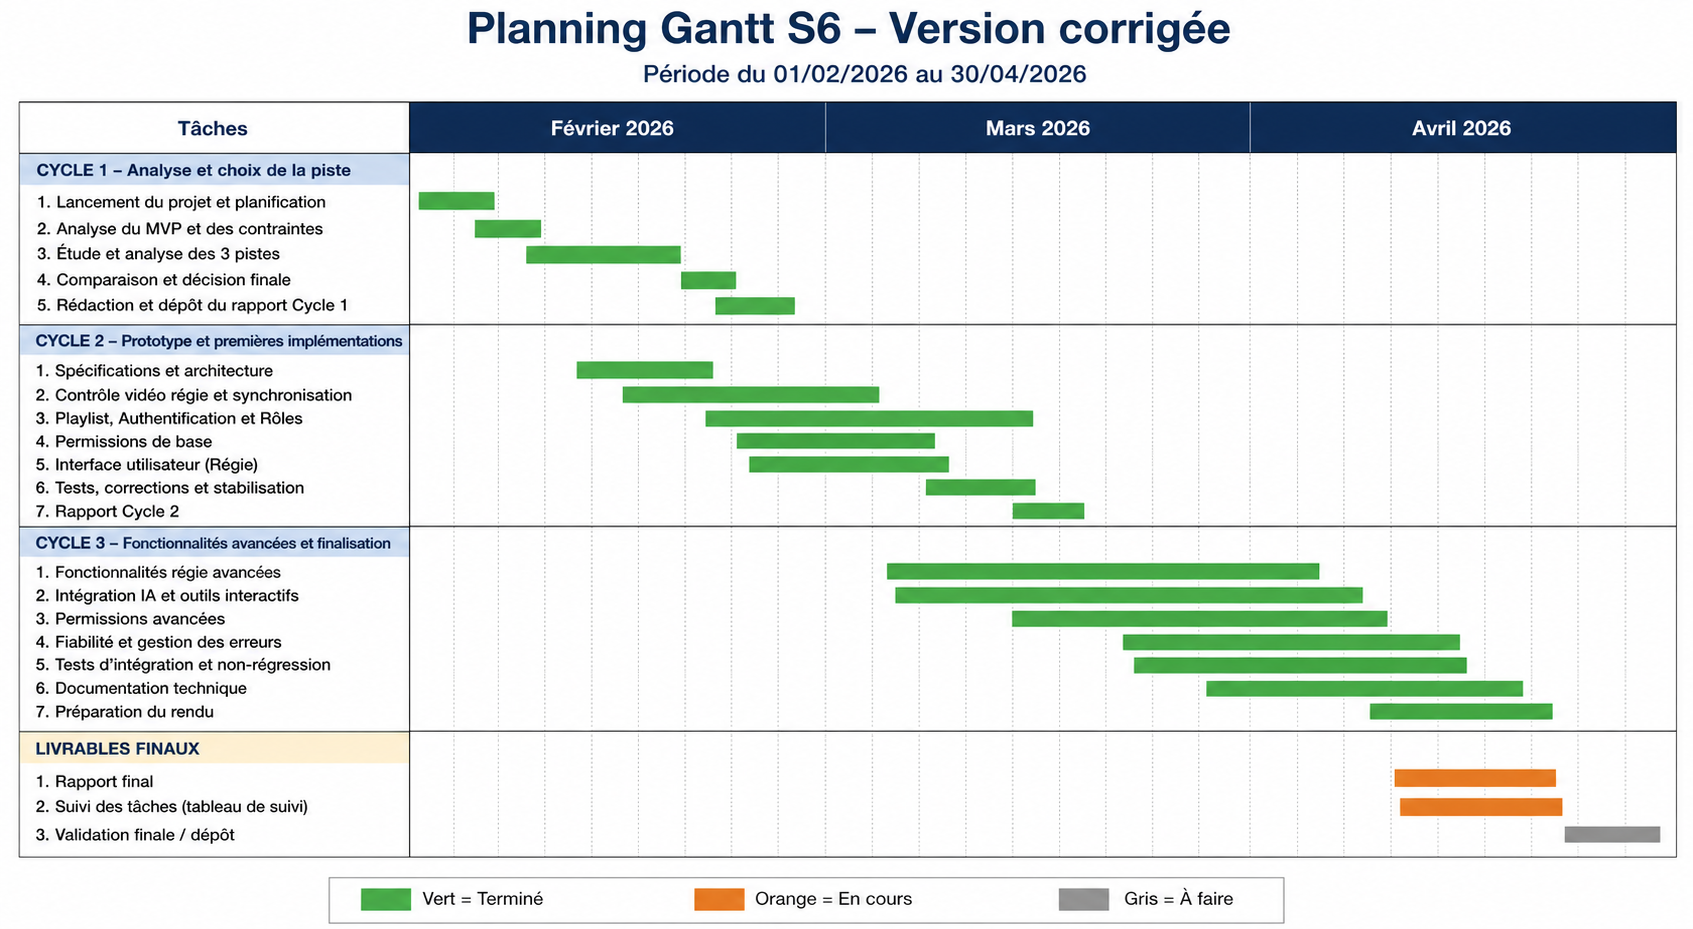
\includegraphics[width=\textwidth]{planning_gantt_s6_corrige.png}
\caption{Diagramme GANTT définitif régissant le phasage synchronisé de la progression d'équipe.}
\end{figure}

\section{A.2 Suivi détaillé des tâches}
Le suivi détaillé des tâches (version complète utilisée pour le pilotage d'équipe) est fourni en annexe sous forme de tableau de suivi dédié.
Cette annexe complète les tableaux synthétiques du corps du rapport.

\end{document}
